%% Manuscript for submission to SIAM 
\documentclass[final,leqno,]{siamltex1213}
% options that require additional .clo file:  
% onetabnum: to number equations consecutively with a single digit, instead of using the section number
% onetabnum: numbers tables consecutively throughout the paper
% onefignum: numbers figures consecutively throughout the paper

\usepackage[text={6in,8in},centering]{geometry} % load first
\usepackage{amsmath}
\usepackage{graphicx}
\usepackage{subfig}

\graphicspath{{figs/}} %  PATH to figure files-- change to ./ for submission

% CUSTOM COMMAND DEFINITIONS
\newcommand{\R}{\mathbb{R}}
\newcommand{\Z}{\mathbb{Z}}
\newcommand{\K}{\mathbb{K}}
\newcommand{\cpu}{\textsc{cpu}}
\newcommand{\gpu}{\textsc{gpu}}
\newcommand{\cuda}{\textsc{cuda}}
\newcommand{\mpi}{\textsc{mpi}}
\newcommand{\bem}{\textsc{bem}}
\newcommand{\bie}{\textsc{bie}}
\newcommand{\fmm}{\textsc{fmm}}
\newcommand{\fmmbem}{\fmm-\bem}
\newcommand{\aca}{\textsc{aca}}
\newcommand{\cpp}{\textsc{c++}}
\newcommand{\blas}{\textsc{blas}}
\newcommand{\sse}{\textsc{sse}}

% CURLY LETTERS
\newcommand{\bigO}{\mathcal{O}}
\renewcommand{\O}[1]{\mathcal{O}(#1)}

% FMM OPERATOR DEFINITIONS
\newcommand{\ptom}{\textsc{p}\texttwooldstyle\textsc{m}\xspace} % P2M
\newcommand{\ltop}{\textsc{l}\texttwooldstyle\textsc{p}\xspace} % L2P
\newcommand{\mtop}{\textsc{m}\texttwooldstyle\textsc{p}\xspace} % M2P
\newcommand{\mtom}{\textsc{m}\texttwooldstyle\textsc{m}\xspace} % M2M
\newcommand{\mtol}{\textsc{m}\texttwooldstyle\textsc{l}\xspace} % M2L
\newcommand{\ltol}{\textsc{l}\texttwooldstyle\textsc{l}\xspace}  % L2L
\newcommand{\ptop}{\textsc{p}\texttwooldstyle\textsc{p}\xspace} % P2P

% MISC THINGS
\newcommand{\ncrit}{N_{\text{CRIT}}}
\newcommand{\pmin}{p_{\text{min}}}
\newcommand{\tsolve}{t_{\text{solve}}}
\newcommand{\csr}{\textsc{csr}}
\newcommand{\nvidia}{\textsc{nvidia}}
\newcommand{\amg}{\textsc{amg}}

% SOLVER DEFINITIONS
\newcommand{\cg}{\textsc{cg}}
\newcommand{\gmres}{\textsc{gmres}}
\newcommand{\fgmres}{\textsc{fgmres}}
\newcommand{\bicgstab}{\textsc{bicgstab}}

% the text 'd' for integrals
\newcommand{\di}[1]{\text{d}#1}
% partial derivatives (frac)
\newcommand{\partiald}[2]{\frac{\partial #1}{\partial #2}}
% partial derivatives (inline)
\newcommand{\partialdi}[2]{\partial #1 / \partial #2}
% \hat{n}
\newcommand{\nhat}{\hat{n}}
% define a vector - undertilde
%\newcommand{\vect}[1]{\utilde{#1}}
% - bold
\newcommand{\vect}[1]{\mathbf{#1}}
% curly L
\renewcommand{\L}{\mathcal{L}}
% curly D
\newcommand{\D}{\mathcal{D}}
% sign
\newcommand{\sign}{\text{sign}}
% basis vectors
\newcommand{\e}{\vect{e}}
% dyadic product
\newcommand{\dyad}[2]{#1 \otimes #2}







\title{INEXACT KRYLOV ITERATIONS AND RELAXATION STRATEGIES WITH FAST-MULTIPOLE BOUNDARY ELEMENT METHOD} 

\author{L. A Barba\thanks{The George Washington University, Washington DC, 20056 
(\email{labarba@gwu.edu})}
\and Simon K. Layton\thanks{If you want to be first author, you have to write ...}}



\begin{document}
\maketitle
%\slugger{sisc}{xxxx}{xx}{x}{x--x}
%slugger should be set to mms, siap, sicomp, sicon, sidma, sima, simax, sinum, siopt, sisc, or sirev

\begin{abstract}
Abstract text here.
\end{abstract}

\begin{keywords}\end{keywords}

\begin{AMS}\end{AMS}


\pagestyle{myheadings}
\thispagestyle{plain}
\markboth{INEXACT KRYLOV ITERATIONS AND RELAXATION STRATEGIES}{WITH FAST MULTIPOLE BOUNDARY ELEMENT METHOD}

\section{Introduction}

Lorem ipsum ...


%% METHODS
\section{Methods for the integral solution of elliptic equations using inexact {\small GMRES}}

\subsection{Boundary-integral solution of the Laplace equation}

To write the Laplace equation, $\nabla^{2}\phi(\vect{x}) = 0$,  in its integral formulation, we use the classical procedure of multiplying by the Green's function and integrating, applying the divergence theorem of Gauss and the chain rule, then dealing with singularities by a limiting process. This results in
%
\begin{equation}\label{eqn:laplace_bem_final}
	\frac{1}{2}\phi + \int_{\Gamma} \phi\partiald{G}{\nhat}\;\di{\Gamma} = \int_{\Gamma}\partiald{\phi}{\nhat}G\;\di{\Gamma},
\end{equation}

\noindent where $G = 1/4\pi r$ is the free-space Green's function for the Laplace equation ($\nabla^{2}G = -\delta$),  $\partiald{\cdots}{\nhat}$ represents the partial derivative in the direction normal to the boundary surface, and the integrals are on the boundary $\Gamma$ of the domain. The boundary element method consists of discretizing the boundary into surface panels and enforcing Equation \eqref{eqn:laplace_bem_final} on a set of target points (collocation version). In its typical form, surface panels take a constant value $\phi_j$, and the surface integrals become sums over $N$ flat surface elements, $\Gamma_j$, resulting in the following discretized equation:
%
\begin{equation}
	\frac{1}{2}\phi_i = \sum_j^{N} \partiald{\phi_j}{\nhat_j}\;\int_{\Gamma}G_{ij}\di{\Gamma_j} - \sum_j^{N} \phi_j\int_{\Gamma}\partiald{G_{ij}}{\nhat_j}\;\di{\Gamma_j}.
\end{equation}

Either the values of the potential or its normal derivative on each panel could be known from boundary conditions, resulting in either first-kind or second-kind integral equations. Finding the remaining unknowns requires solving a system of linear equations $A\vect{x}=\vect{b}$, where the elements of the coefficient matrix are
%
\begin{equation}
	A_{ij} = 
	\begin{cases}
		\int_{\Gamma} G_{ij}\;\di{\Gamma_j}, & \phi\;\text{given on panel}\;j \\
		\int_{\Gamma} \partiald{G_{ij}}{\nhat_j}\;\di{\Gamma_j}, & \partiald{\phi}{\nhat}\;\text{given on panel } j
	\end{cases}
\end{equation}

\noindent
and $\vect{b}$ is formed with the known terms: e.g., if $\phi$ is given on panel $j$, then $\phi_j\int_{\Gamma_j}\partialdi{G_{ij}}{\nhat_j}\;\di{\Gamma_j}$ will appear in the term $b_i$ on the right-hand side of the linear system.

Inserting for $G_{ij}$ and $\partialdi{G_ij}{\nhat_j}$ in terms of $1/r$ and $\nhat_j\cdot\nabla(1/r)$ results in
%
\begin{eqnarray}
	\label{eqn:laplace_bem_G}\int_{\Gamma} G_{ij}\;\di{\Gamma_j} & = & \int_{\Gamma} \frac{1}{|\vect{x}_i-\vect{x}_j|} \;\di{\Gamma_j} \\ 
	\label{eqn:laplace_bem_dGdn}\int_{\Gamma} \partiald{G_{ij}}{\nhat_j}\;\di{\Gamma_j} & = & \int_{\Gamma}\frac{d\vect{x}\cdot\nhat_j}{|\vect{x}_i-\vect{x}_j|^{3}}\;\di{\Gamma_j}
\end{eqnarray}

The next step is to apply an appropriate numerical integration scheme in order to generate all the terms of the coefficient matrix.

\subsection{Boundary-integral solution of the Stokes equation}

\subsection{Numerical integration methods}

\subsection{Krylov subspace methods}

\subsection{Fast multipole method}

%$ RESULTS
\section{Results}

\subsection{Inexact {\small GMRES} for the solution of Laplace's equation}
To start, we looked at grid-convergence using a sphere with constant potential and charge on the surface: $\phi = \partialdi{\phi}{\nhat} = 1$.


\begin{center}
\begin{figure}[b]
	\subfloat[][128 panels]{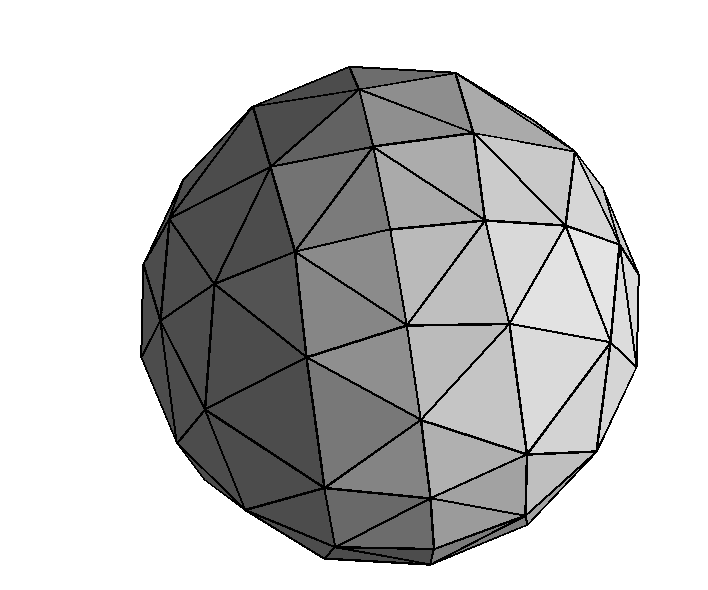
\includegraphics[natwidth=4.73in,width=0.45\textwidth]{sphere128.pdf}\label{fig:sphere128}}\qquad
	\subfloat[][2048 panels]{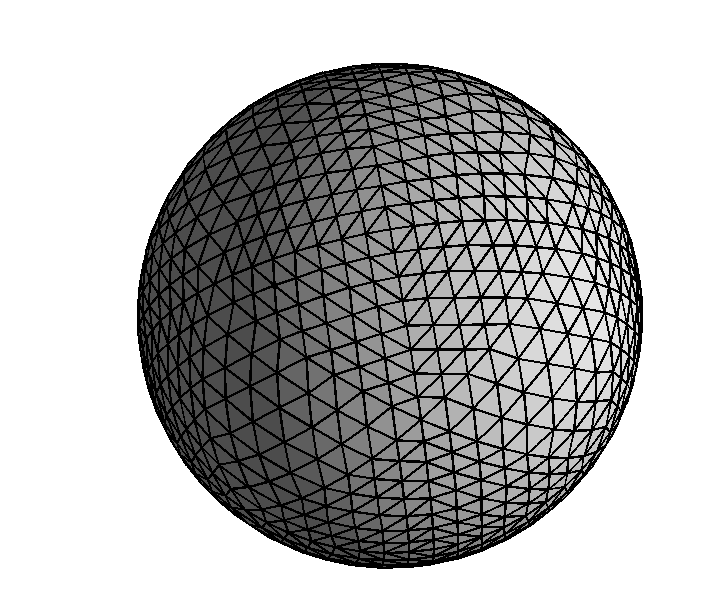
\includegraphics[natwidth=4.73in,width=0.45\textwidth]{sphere2048.pdf}\label{fig:sphere2048}}
	\caption{Triangular discretizations of a spherical surface.}
	\label{fig:glob_spheres}
\end{figure}
\end{center}

\section{Conclusion} 



 
%% Acnowledgements

%% Bibliography


\end{document}
%% end of file `docultex.tex'
